% !TEX encoding = UTF-8 Unicode

\documentclass[a4paper]{article}

\usepackage{color}
\usepackage{url}
\usepackage[T2A]{fontenc} % enable Cyrillic fonts
\usepackage[utf8]{inputenc} % make weird characters work
\usepackage{graphicx} % potrebno za sliku

\usepackage{makecell} % potrebno za formatiranje tabele
%\usepackage{tabu}

\usepackage{amsmath} % potrebno za matematiku
\usepackage{amsfonts}

\usepackage[english,serbian]{babel}
%\usepackage[english,serbianc]{babel} %ukljuciti babel sa ovim opcijama, umesto gornjim, ukoliko se koristi cirilica

\usepackage[unicode]{hyperref}
\hypersetup{colorlinks,citecolor=green,filecolor=green,linkcolor=blue,urlcolor=blue}

%\newtheorem{primer}{Пример}[section] %ćirilični primer
\newtheorem{primer}{Primer}[subsection]
\newtheorem{defn}[primer]{Definicija}

\begin{document}

\title{Diffie-Hellman algoritam\\ \small{Seminarski rad u okviru kursa\\Tehničko i naučno pisanje\\ Matematički fakultet}}

\author{Dunja Milenković\\ mi22056@alas.matf.bg.ac.rs\and Jana Vuković\\mi22124@alas.matf.bg.ac.rs\and Lazar Nikolić\\mi22164@alas.matf.bg.ac.rs\and Sofija Janevska\\mi22035@alas.matf.bg.ac.rs }
\date{15.~novembar 2022.}
\maketitle

\abstract{
    Ovde će ići abstrakt
}

\tableofcontents

\newpage

\section{Uvod}
\label{sec:uvod}
Sve rasprostranjenija upotreba interneta širom sveta donosi sa sobom, kako značajne prednosti u načinu istraživanja, rada, povezivanja i sl. tako i povećan rizik od nebezbedne komunikacije i razmene podataka. Bilo da se radi o individualnim, privatnim razmenama informacija između ljudi ili rada nekih od najvećih državnih institucija, bezbedna i neometana interakcija i komunikacija među korisnicima na internetu je od presudnog značaja. Glavni problem nastaje kada spoljni korisnik koji nije predviđen kao deo veze pokuša da je prekine i dođe do određenih informacija koje su originalno bile namenjene jednom od povezanih korisnika. Upravo rešavanjem ovakvih problema bavi se \textbf{kriptografija}.

Kriptografija je oblast koja razvija tehnike koje omogućavaju zaštićenu i efikasnu digitalnu komunikaciju \cite{cryptography}. Bez nje, komunikacija nebezbednim i nepoverljivim kanalima, što uključuje sve vrste mreža, a pogotovo internet, ne bi bila moguća. U ovom radu bavićemo se jednom od tehnika kriptografije koja se naziva \textbf{Diffie-Hellman algoritam} %tj. \textbf{Diffie-Hellman protokol}
i predstavićemo način rada algoritma, njegova osnovna svojstva, primene, prednosti i mane.

\section{Osnove Diffie-Hellman algoritma}
Glavna klasifikacija kriptografskih algoritama deli ih na kriptografiju privatnog ključa (eng. secret key cryptography), kriptografiju javnog ključa (eng. public key cryptography) i heš funkcije (eng. hash functions) \cite{cryptography}. Kako je Diffie-Hellman protokol predstavnik asimetrične kriptografije, nju ćemo posebno izdvojiti i definisati.

\textbf{Kriptografija javnog ključa} ili \textbf{asimetrična kriptografija} podrazumeva korišćenje dva ključa – jednog za šifrovanje i drugog za dešifrovanje koda. „Tvorcima“ tj. pokretačima asimetrične kriptografije smatraju se \textbf{Whitfield Diffie} (Vitfild Difi) i \textbf{Martin Hellman} (Martin Helman), dok je Ralph Merkle (Ralf Merkl) takođe dao svoj doprinos ovoj oblasti radom na distribuciji javnog ključa \cite{Diffie-Hellman}. Njihova saradnja rezultirala je objavom zajedničkog rada pod nazivom ,,Novi pravci u kriptografiji‘‘ (eng. "New Directions in Cryptography"), novembra 1976. godine. U njemu su opisane osnove Diffie-Hellman algoritma, koji je upravo otud i dobio naziv. %Diffie i Hellman su 2015. godine dobili Tjuringovu nagradu za svoja dostignuća u oblasti kriptografije. 

U spomenutom radu, Diffie-Hellman algoritam opisan je kao algoritam koji koristi dva ključa i tako omogućava korisnicima bezbednu komunikaciju bez potrebe za deljenjem privatnog ključa. Takođe, simetrična kriptografija omogućava postojanje digitalnih potpisa tj. autentifikacije pošiljaoca poruke. Osnovni princip na kome funkcioniše jeste korišćenje tzv. jednosmernih matematičkih funkcija (eng. one-way functions), koje se lako izračunavaju u jednom smeru, dok isto ne važi i za njihove inverzne funkcije \cite{cryptography}. Na ovaj način omogućeno je postojanje javnog ključa, bez rizika da ga treći korisnik koji nije predviđen kao deo mreže može zloupotrebiti. 



\section{Algoritam}
\label{sec:algoritam}

Pre početka razmene ključeva, uspostavljaju se 2 javno poznata broja: $p$ i $g$.
\begin{itemize}

    \item $p$ - \emph{bezbedan prost broj} i modulo po kom radimo, preporuka je da 
        to bude broj dužine 2048 bita (broj reda $10^{616}$) \cite{logjam}
    \item $g$ - generator, mora da bude \emph{primitivni koren} od $p$

\end{itemize}

\begin{defn}
    \emph{Bezbedan prost broj}: $p$ je bezbedno prost ako može da se izrazi kao $p = 2q + 1$ gde je $q$ takođe prost broj. 
    $q$ je Sofija Žermen prost (eng. \emph{Sophie Germain prime}). 
\end{defn}
Ovo je bitno kako bi se izbegao specifičan napad na Diffie-Hellman --- 
Silver-Polig-Hellman algoritam (eng. \emph{Silver-Pohlig-Hellman algorithm}) \cite{pohlig-hellman}

\begin{defn}
    \emph{Primitivni koren}: $g$ je primitivni koren po modulu $p$ ako za
    svaki celi broj $a$ koji je uzajamno prost sa $p$ postoji celi broj $k$ tako da je
    \[g^k \equiv a \mod p\]
    Takvo $k$ se naziva indeks ili diskretni logaritam od $a$ sa osnovom $g \mod p$.
\end{defn}


\subsection{Koraci algoritma}
\label{subsec:koraci_algoritma}

\begin{defn}
    Najmanji pozitivni ostatak nekog $x$ po modulu $p$ je najmanji pozitivni celi broj $a$ tako da je 
    \[x \equiv a \mod n\]
\end{defn}

Recimo da Anastasija i Boban žele da razmene ključeve.
\begin{itemize}
    \item Pretpostavljamo da su se Anastasija i Boban već dogovorili oko brojeva $g$ i $p$
%    \item Anastasija nasumično bira neki tajni broj $x \in \mathbb{N}$ i izračuna njegov \emph{najmanji pozitivni ostatak} 
%        (objašnjeno kasnije), čime dobija  $a$, ovo je njen privatni ključ
    \item Anastasija računa \emph{najmanji pozitivni ostatak} nasumično odabranog broja $x \in \mathbb{N}$,
        čime dobija njen privatni ključ $a$, zatim računa njen javni ključ $A = g^a \mod p$
%    \item Zatim kalkuliše njen javni ključ koji je jednak $A = g^a \mod p$ 
    \item Boban će uraditi isto, nakon čega poseduje privatni ključ $b$ i javni ključ $B = g^b \mod p$
    \item Anastasija i Boban sada razmene njihove javne ključeve (privatni ključevi ostaju tajni)
    \item Anastasija sada poseduje svoje ključeve, kao i Bobanov javni ključ
    \item Ona će izračunati tajni broj $K = B^a \mod p$. Ako zamenimo $B$, videćemo da je
        \begin{align*}
%            K = (g^b \mod p)^a \mod p &=\\ (g^b)^a \mod p &=\\ g^{ab} \mod p
            K = (g^b)^a \mod p &=\\ g^{ab} \mod p
        \end{align*}
    \item Boban sada poseduje svoje ključeve i Anastasijin javni ključ
    \item On će istim postupkom kao i Anastasija pronaći $K$:
        \begin{align*}
%            K = A^b \mod p &=\\ (g^a \mod p)^b \mod p &=\\ (g^a)^b \mod p &=\\ g^{ab} \mod p
            K = A^b \mod p &=\\ (g^a)^b \mod p &=\\ g^{ab} \mod p
        \end{align*}
\end{itemize}

%NOVA TABELA

\begin{table}
    \begin{center}
    \begin{tabular}{ |c|c|c|c| }
        \hline
        Trenutni korak & Anastasija zna & Javno poznato & Boban zna \\
        \hline
        Početak algoritma &  & $g, p$ &  \\
        \hline
        \makecell{Svako računa\\svoj ključ} & $a, A=g^a \mod p $ & $g, p$ & $b, B=g^b \mod p$ \\
        \hline
        \makecell{Razmena\\javnih ključeva} & $a, A, B$ & $g, p, A, B$ & $b, B, A $ \\
        \hline
        \makecell{Svako računa isto, \\ tajno K} &
        \makecell{{$\!\begin{aligned}
            a, A, B,\\K=B^a \mod p\\=g^{ab} \mod p
        \end{aligned}$} } &
        \makecell{$g, p, A, B$} &
        \makecell{{$\!\begin{aligned}
            b, B, A,\\K=A^b \mod p\\=g^{ab} \mod p
        \end{aligned}$}\\}\\
        \hline
    \end{tabular}
    \caption{\textbf{Tajnost promenljivih u toku algoritma}}
    \label{table:tajnost_promenljivih}
    \end{center}
\end{table}

Primetimo da će i Anastasija i Boban izračunati isti broj $K$ (\ref{slika:boje}).  
$K$ predstavlja ključ za enkripciju ključeva (engl. \emph{Key-Encryption Key (KEK)}). 
Pomoću tog ključa mogu sinhrono da razmene novi ključ za enkripciju sadržaja 
(engl. \emph{Content-Encryption Key (CEK)}) i da nastave komunikaciju pomoću njega. \cite{dhstandard}

Neko ko je prisluškivao ovoj razmeni zna $p$, $g$, $g^a$ i $g^b$ (\ref{table:tajnost_promenljivih}).
Da bi od ovih brojeva pronašao $K$, on mora da izračuna vrednost $a$ ili $b$, 
problem koji se zove \emph{komputacioni Diffie-Hellman problem} (engl. \emph{computational Diffie-Hellman problem (CDH)}).

\begin{figure}
\centering
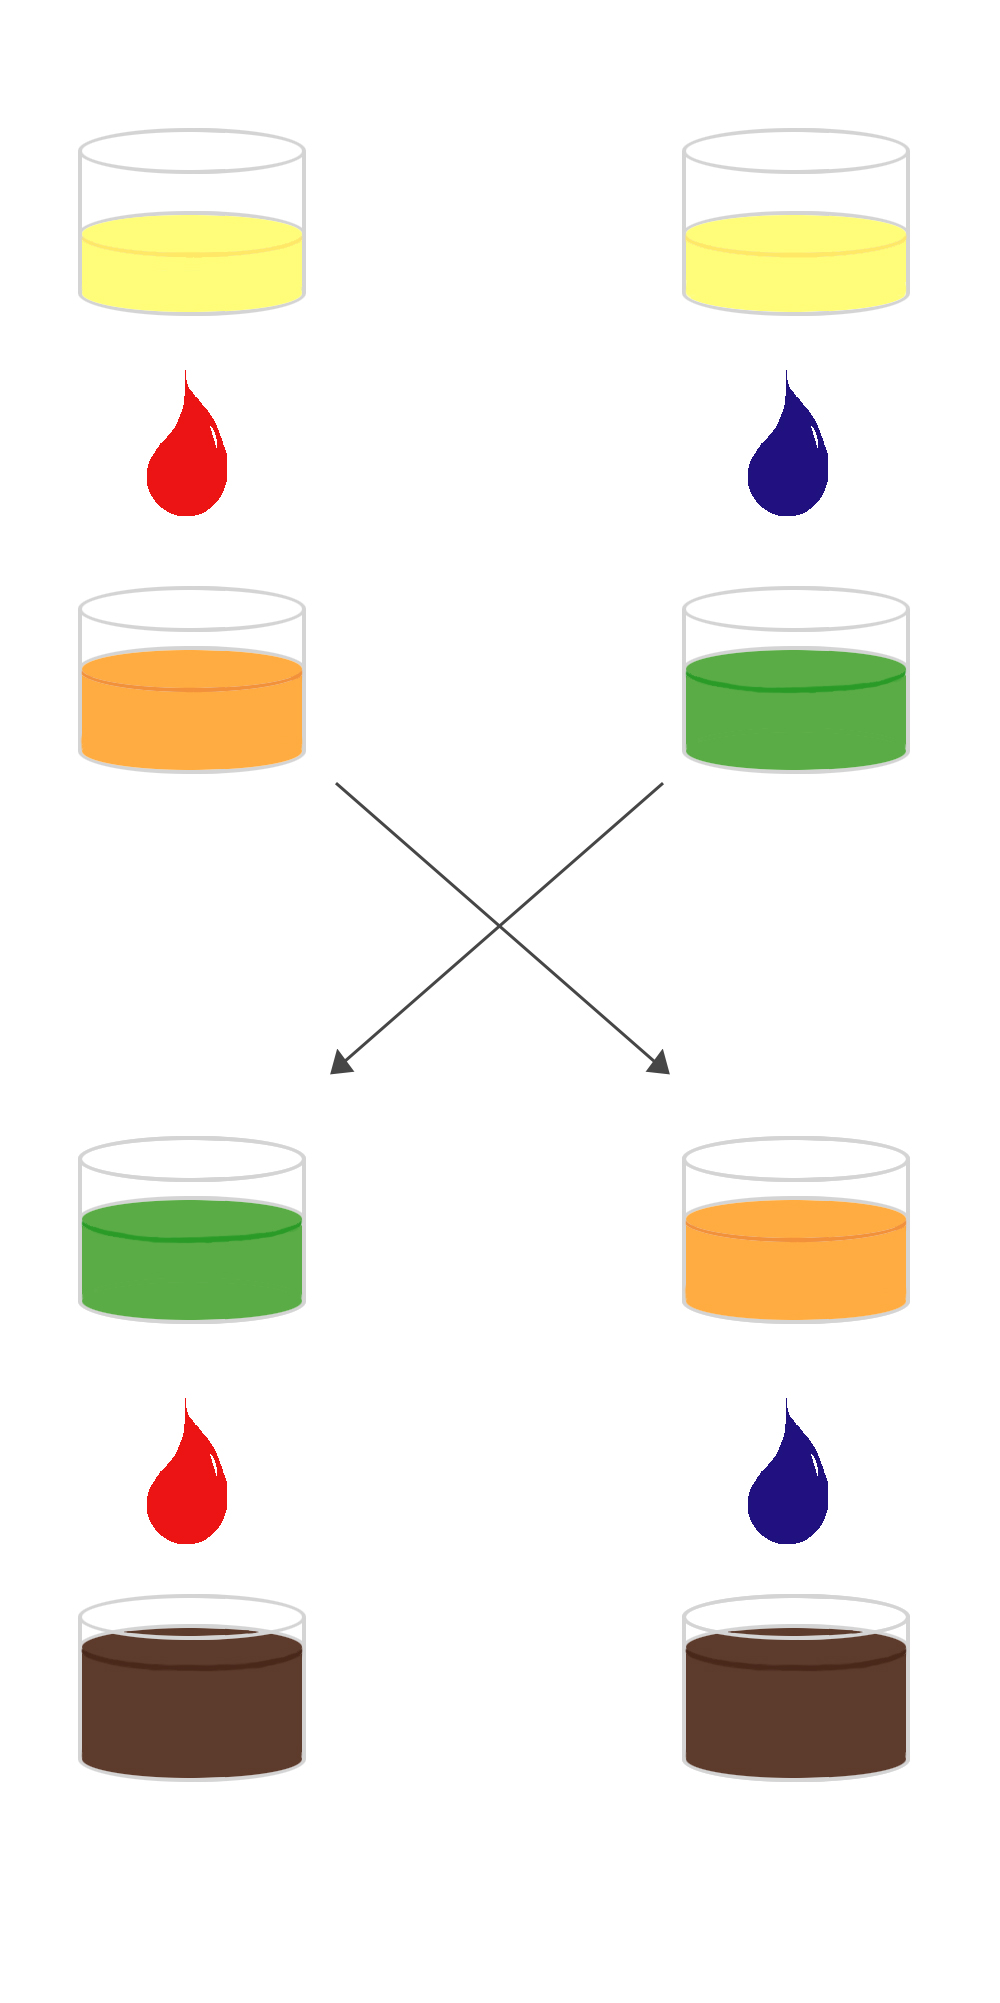
\includegraphics{Boje.jpg}
\caption{\textbf{Slikoviti prikaz Diffie-Hellman algoritma}}
\label{slika:boje}
\end{figure}

\subsection{Problemi oslonci}
\label{subsec:problemi_oslonci}

Neka $G$ bude ciklična grupa reda $q$, sa generatorom $g$. %Drugačije rečeno, svaki broj $x$ iz $G$ je 
%kongruentan sa nekim $g^k$, gde je $k$ neki celi broj tako da je $0 \leq k \leq q - 1$.
%\[x = g^k\]
Ako znamo $g$ i $k$, lako možemo izračunati $x$. Međutim, ako znamo $x$ i $g$, pronalaženje $k$ je veoma teško, 
i to je zapravo problem diskretnog logaritma.

\begin{defn}
Problem diskretnog logaritma u cikličnoj grupi $G$ reda $q$ je pronalaženje broja $k$, $0 \leq k \leq q - 1$ 
tako da $x = g^a$, za neko $g$ i $x$.
\end{defn}

%Ako možemo da rešimo problem diskretnog logaritma, možemo da nađemo i tajni broj $K$ iz Diffie-Hellman ako znamo oba javna ključa.
%Obrnuto nije dokazano: ako možemo da pronađemo tajni broj $K$, ne mora da znači da možemo rešiti bilo koji problem 
%diskretnog logaritma.

Ne treba da pretpostavimo da je diskretni logaritam jedini način da se razbije Diffie-Hellman. 
Dovoljna je bilo koja metoda koja može da pronađe $g^{ab}$ iz $g^a$ i $g^b$, i otud uvođenje sledećeg problema:

\begin{defn}
    Neka $a,b\in \mathbb{Z}\setminus q\mathbb{Z}$ ($a$ i $b$ su u nekoj cikličnoj grupi reda $q$),
    i neka $A = g^a$ i $B = g^b$.
    \textbf{Komputacioni Diffie-Hellman problem} (CDH) je problem nalaženja $g^{ab}$ ako znamo $A$ i $B$ u cikličnoj grupi
    $G = \langle g \rangle$ reda $q$.
\end{defn}

Na težini ovog problema se oslanja bezbednost Diffie-Hellman šeme.
Najefikasnije rešenje za koje znamo je da rešimo problem Diskretnog Logaritma 
ali još uvek nije dokazana ekvivalencija između njih. \cite{dlproblem}

Takođe slična je i ElGamal enkripcija o kojoj će biti reči kasnije. Ona se oslanja na sledeći problem:

\begin{defn}
    Neka $a,b,c\in \mathbb{Z}\setminus q\mathbb{Z}$ i $A = g^a$, $B = g^b$. Sa verovatnoćom $\frac{1}{2}$ postavimo $C = g^c$, 
    a inače $C = g^{ab}$. Odlučujući Diffie-Hellman problem (engl. \emph{Decisional Diffie-Hellman problem (DDH)}) je problem
    odlučivanja da li je $C = g^{ab}$, ako znamo $\langle g \rangle$ i $A, B, C$.
\end{defn}

Ako znamo da rešimo komputacioni Diffie-Hellman problem, lako je rešiti odlučujući Diffie-Hellman problem.
Obrnuto ne važi. \cite{ddh-vs-cdh}


\subsection{Primer Diffie-Hellman algoritma na konkretnim vrednostima}
\label{sec:primerDH}

Algoritam opisan u prethodnim poglavljima, primenjen na vrednostima konkretizovanim kroz interakciju dva korisnika izgleda ovako:
\begin{itemize}
  \item Neka je izabrani prost broj $q=353$.
  \item Prost koren za ovu vrednost je $\alpha=3$. 
  \item Korisnik A bira tajni ključ $X_A=97$. \item Korisnik B bira tajni ključ $X_B=233$.
  \item Korisnik A izračunava javni ključ $Y_A=3^{97}\mod353=40$.
  \item Korisnik B izračunava javni ključ $Y_B=3^{233}\mod353=248$.
  \item Korisnici A i B razmenjuju javne ključeve $Y_A$ i $Y_B$, nakon čega oba korisnika mogu da izračunaju tajni ključ $K$.
  \item Korisnik A tajni ključ izračunava po formuli: $$K=(Y_B)^{X_A}\mod353=248^{97}\mod353=160$$
  \item Korisnik B tajni ključ izračunava po formuli: $$K=(Y_A)^{X_B}\mod353=40^{233}\mod353=160$$
\end{itemize}

Po samoj definiciji algoritma možemo slobodno pretpostaviti da napadač na raspolaganju ima samo podatke o vrednosti izabranog prostog broja i njegovog prostog korena, kao i vrednosti javnih ključeva korisnika A i B. Dakle, napadač zna da je: \\\centerline{$q=353$, $\alpha=3$, $Y_A=40$ i $Y_B=248$.}

S obzirom da su radi jednostavnosti izabrani brojevi u ovom primeru veoma mali, napadač može da pokuša i teorijski uspe da otkrije vrednost tajnog ključa $K$, primenjujući čistu metodu grube sile ("brute force").

Da bi napadač otkrio vrednost tajnog ključa $K$, neophodno je da otkrije bar jednu vrednost koja će zadovoljavati jednačinu za izračunavanje tajnog ključa koju koriste korisnici. Koristeći informacije koje su mu poznate, napadač može da rekonstruiše kako igledaju te jednačine, a potom pokuša da ih reši metodom grube sile: \\\centerline{$Y_A=3^a\mod353=40$ ili $Y_B=3^b\mod353=248$.}

Metoda grube sile u ovom slučaju podrazumeva stepenovanje trojke sve dok dobijena vrednost po modulu 353 ne postane 40 ili 248.

Jednačina biva zadovoljena kada je eksponent $a=97$. Sa ovim saznanjem, napadač izračunava vrednost tajnog ključa $K$ i dešifruje podatke deljene između korisnika A i B.

Zbog ovoga se u Diffie-Hellman algoritmu koriste vrednosti koje su značajno veće. U tom slučaju razbijanje algoritma grubom silom postaje krajnje nepraktično.
 

\section{ElGamalov sistem enkripcije}
\label{sec:Elgamal}
Nakon što su Diffie i Hellman uveli koncept kriptografije javnog ključa, mnogo istraživača pokušalo je da pronađe efikasniji sistem enkripcije zasnovan na Diffie-Hellman algoritmu (linkovi 6,7,9 iz originalnog rada). Za razliku od npr. RSA sistema (9) koji se oslanja na kompleksnost faktorisanja velikih celih brojeva, ElGamalov sistem zasnovan je na kompleksnosti izračunavanja vrednosti diskretnih logaritama.

Glavne celine koje se uočavaju u koracima ElGamalovog algoritma su:
\begin{enumerate}
    \item Javno su poznata dva cela broja - prost broj $q$ i njegov prost koren $\alpha$ koji je ceo broj.
    \item Anastasija generiše par ključeva (privatni i javni).\begin{itemize}
        \item Bira privatan ključ $X_A$, ali takav da je $1<X_A<q-1$.
        \item Izračunava javni ključ po formuli $Y_A=\alpha^X_A\mod q$
        \item Privatni ključ je $X_A$, a javni ključ je ${q,\alpha,Y_A}$
    \end{itemize}
    \item Boban šifruje poruku koristeći Anastasijin javni ključ.\begin{itemize}
        \item Predstavi poruku kao ceo broj $M$ iz domena $[0,q-1]$.
        \item Odabere proizvoljan ceo broj $k$ iz domena $[1,q-1]$.
        \item Izračuna privremeni ključ za jednokratnu upotrebu, po formuli: $K=Y_A^k\mod q$.
        \item Konačno, broj kojim je reprezentovana poruka šifruje kao par celih brojeva $(C1,C2)$, i to: $C1=\alpha^k \mod q$, i $C2=KM\mod q$.
    \end{itemize}
    \item Anastasija dešifruje dobijenu šifrovanu poruku $M$ koristeći svoj privatni ključ.\begin{itemize}
        \item Uzima jednokratni ključ $K=C_1^{X_A}\mod q$.
        \item Izračunava originalnu poruku $M$ po formuli $M=(C_2K^{-1})\mod q$.
    \end{itemize}
\end{enumerate}

 Dakle, Elgamalov algoritam sastoji se iz tri glavne tačke - generisanje ključa, enkripcija i dekripcija. U datom postupku, Boban želi neometano da pošalje poruku Anastasiji, diskretno i bez mešanja trećeg lica. Na prelazu između prvog i drugog koraka Anastasija šalje Bobanu javni ključ ${q,\alpha,Y_A}$ koji je sama formirala. Na prelazu između drugog i trećeg koraka Boban šalje Anastasiji uređeni par celih brojeva $(C1,C2)$ kojim je šifrovao poruku $M$ koju želi da joj pošalje. Na osnovu dobijenog para Anastasija prevodi poruku. 
 
 Ukoliko je poruka previše dugačka i neophodno ju je razbiti na više delova, za enkripciju svakog pojedinačnog dela neophodno je nasumično izabrati različito $k$ (izbor ove vrednosti dešava se u drugoj tački trećeg koraka u navedenom ElGamal algoritmu). ElGamal algoritam je siguran ukoliko se za enkripciju koriste dovoljno veliki brojevi. Preporučena minimalna veličina za nasumično izabran prost broj $q$ je trista cifara.

\subsection{Dokaz ispravnosti ElGamalovog algoritma}
Prema definiciji ElGamalovog algoritma, privremeni ključ za jednokratnu upotrebu računa se po formuli $K=Y_A^k\mod q$. Po Diffie-Hellman definiciji, $Y_A=\alpha^{X_A}\mod q$. Kada se ovaj izraz zameni u početnoj formuli, dobije se $K=(\alpha^{X_A}\mod q)^k\mod q =\alpha^{kX_A}\mod q$. Po ElGamalovoj definiciji, $C_1=\alpha^k\mod q$. Kada se ovaj izraz zameni u prethodnoj formuli, dobije se $K=C_1^{X_A}\mod q$, čime je dokazano da i Anastasija i Boban mogu izračunati istu vrednost privremenog ključa na osnovu sebi raspoloživih podataka.

Boban formira uređeni par celih brojeva kojima šifruje poruku M. Po definiciji ElGamal algoritma, on će drugi broj formirati po formuli $C2=KM\mod q$. Anastasija če dobiti uređeni par i po definiciji će poruku dešifrovati formulom $M=(C_2K^{-1})\mod q$. Ukoliko u ovu formulu zamenimo formulu po kojoj Bobam formira vrednost $C_2$, dobija se izraz $M=((KM\mod q)K^{-1})\mod q=(KMK^{-1})\mod q=M\mod q=M$, čime je dokazano da Anastasija može da na osnovu dostupnih podataka dešifruje poruku koju joj je poslao Boban.

\subsection{Primer ElGamal algoritma na konkretnim vrednostima}
Algoritam opisan u prethodnim poglavljima, primenjen na vrednostima konkretizovanim kroz interakciju dva korisnika izgleda ovako:
\begin{itemize}
  \item $q=19$, $\alpha=10$. 
  \item $X_A=5$, $Y_A=\alpha^{X_A}\mod q=10^5\mod 19=3$.
  \item $M=17$, $k=6$.
  \item $K=Y_A^k\mod q=3^6\mod 19=7$.
  \item $C1=\alpha^k \mod q=10^6\mod 19=5$
  \item $C2=KM\mod q=7\cdot17\mod 19=5$
  \item $K=C_1^{X_A}\mod q=11^5\mod 19$
\end{itemize}
... jos malo lol

\section{Diffie-Hellman pod napadom}
Razmenu tajne Anastasije i Bobana napadač želi da spreči, to može učiniti na različite načine. Zavisno od cilja - da li želi da dobije deljene informacije ili da spreči Bobana u dobijanju istih, mi delimo napade Diffie-Hellman protokola na sledeći način:
\begin{itemize}
\item Autsajder (eng. \emph{Outsider}) napad - I u ovom tipu napada napadač ometa DH protokol, ali na način na koji dobija informacije. On dodaje, briše, ponavlja poruke kako bi se domogao informacija do kojih ne može da dođe isključivo uz pomoć javnog ključa.
\item Insider napad - Ukoliko Anastasija ili Boban odluči da objavi tajnu, to može učiniti time što će napraviti protokol koji se može lako razbiti odnosno svako ko vidi javni ključ može lako zaključiti šta je tajna.
\item DoS (eng. \emph{Denial of Service}) - Napadač pokušava da omete izvršenje DH protokola onesposobljavanjem mreže, računara.
\end{itemize}


\subsection{Čovek u sredini}
Aleksandar se sprema za napad. Kako je u mogućnosti da briše i postavlja poruke, on će spremiti dva ključa $g^{a'}$ i $g^{b'}$ koje će zameniti sa $g^{a}$ i $g^{b}$ redom. U slučaju kada nisu izvršili autentifikaciju Anastasija i Boban misle da imaju ispravne ključeve koje će koristiti da generišu $g^{ab}$. Pretpostavimo da Anastasija želi da pošalje poruku m, i da je $ENC_{K}(x)$ simetrična enkripcija od $x$ koristeći ključ $K$. Prikazaćemo kako se dalje odvija napad u tri koraka od kojih prva dva predstavljaju prisluškivanje, a u trećem koraku dolazi do zamene poruka.

1. Anastasija šalje $ENC_{g^{ab’}}(m)$

2. Aleksandar presreta poruku i dešifruje je. $g^{ab'}$ mu je poznata, tako da lako dolazi do poruke $m$.

3. Aleksandar sprečava enkriptovanu poruku m da stigne do Bobana i umesto nje šalje $ENC_{g^{a'b}}(m')$ pri čemu $m'$ može biti bilo šta.

Privatnost je narušena, a samim tim je i šema šifrovanja kompromitovana. Za ovaj tip napada Aleksandar mora da bude izuzetno moćan, ponaročito u situacijama kada autentifikacija postoji. Tada je potrebno da Aleksandar presreta i vrši izmenu nad svakom autentifikovanom porukom kako Anastasija i Boban ne bi primetili da je Aleksandar izvršio napad.

Postoji još jedan oblik napada Čovek u Sredini. Ovaj oblik obuhvata samo priskluškivanje odnosno Aleksandar je u mogućnosti da vidi samo poruke. Glavni problem pri ovom napadu predstavlja računarska Diffie-Hellman pretpostavka (CDH) koja govori da za ciklični skup $G$ reda $q$ imamo $g$, $g^{a}$ i $g^{b}$ pri čemu su $g$ i $a, b\in$ \{0, 1,...,q - 1\}. Zbog činjenice da je računanje logaritma sa bazom $g$ u skupu $G$ sa proizvoljnim vrednostima teško dolazimo do zaključka da je CDH izuzetno komplikovan proces. Kada bi postojao efikasniji način da dođemo do vrednosti $a$ i $b$ postupak dešifrovanja poruka bi se sveo na sledeće korake: izračunavanje $a$ uzimanjem logaritamske vrednosti izraza $g^{a}$, a potom ubacivanje iste vrednosti u $g^{ab}$ tj. $(g^{b})^{log_g(g^{a})}$. 
\subsection{Početnička greška}
Ukoliko Anastasija ili Boban izabere $g^{a}=1$ odnosno $g^{b}=1$ onda će $g^{ab}$ biti jednako 1. S obzirom da je razmena tajnog ključa javna, svako ko vidi isti je u mogućnosti da uoči ovu grešku. Postoji i druga greška koja se može javiti, a to je kada je $g^{a}=g$. Jedna od prednosti koje RSA (Rivest–Shamir–Adleman) kriptosistem ima jeste zahtev da svako $a$ i $b$ zadovoljavaju uslov dužine $p$ odnosno $a,b\geq2^{p-1}$, pri čemu dužinu definišimo kao $k$ za koje broj $n$ zadovoljava $n\geq2^{k}$. 

Pretpostavimo da su $a$ i $b$ ispravni i da $g^{ab}$ nije lako odrediti. Ukoliko proveru ne vrši biće sposobno da logički zaključi da se pojavila greška, već računar kod kojeg DH protokol nije ispravno implementiran onda napadač Veljko sa lakoćom presreta $g^{a}$ i $g^{b}$, i zamenjuje obe vrednosti sa $g^{v}=1$. Samim tim $g^{ab}=1$ i protokol je ranjiv samo ako računar ne detektuje grešku. Isti argument važi za vrednosti oblika $g^{\alpha*a*(p-1)}$ gde je $\alpha\geq1$
\subsection{Lažno predstavljanje}
Postoji više načina na koje Miloš može da prevari Anastasiju koja misli da prima Bobanove poruke. Jedan od načina jeste ponovno slanje Bobanovih poruka. Recimo da su Anastasija i Boban zajedno i da joj je Boban poslao poruku: "Volim te". Nakon par godina nesrećnog braka i teškog raskida, Miloš 
 bi samo ponovio Bobanovu poruku. Naravno, Miloš mora da bude izuzetno moćan kako bi izvršio ove tipove napada.

Ukoliko Miloš želi da dovede Bobana u još goru situaciju on će presresti njegovu poruku i poslati je Mileni. Naši primeri su samo mali delić beskonačnih mogućnosti koje ovaj napad pruža.


\subsection{DoS napad}
Petrov cilj je da preoptereti server lažnim zahtevima koristeći činjenicu da su serveri memorijski ograničeni i same sposobnosti računara. DH protokol je podložan sledećim DoS tipovima napada:
\begin{itemize}
\item Memorijski - Najlakši način na koji se server može zaštiti od ovoga jesu kriptografske zagonetke. Inicijatori konekcije su primorani da pre svakog poslatog zahteva odnosno poruke odrade jednu zagonetku. One ne troše puno vremena za normalne korisnike, ali za Petra one su noćna mora. Kako bismo u potpunosti zaštitili server potrebno je da svaka zagonetka ima vremenski interval u toku kojeg morate odgovoriti na nju. Pritom je bitno da naglasimo da $t_1 \neq t_2$ gde je $t$ spomenuti vremenski interval. 
\item Računarski - Petar se vraća, ovoga puta je naoružan sa gomilu nasumično generisanih ključeva koji nemaju ništa drugo za cilj sem da preopterete Bobanov računar koji pokušava da izračuna tajni zajednički DH ključ koristeći prebrojivo mnogo lažnih ključeva. 
Bitno je da naglasimo da je potrebno odrediti vremenski period za koji konekcija sa serverom postoji. Ukoliko ona traje beskonačno dugo, server je podložan DoS napadu.
\end{itemize}

\section{Primene na bezbednosnim protokolima}
\label{sec:primene}

Diffie-Hellman algoritam ima široku primenu na različitim internet protokolima, od kojih su najvažniji SSL, SSH i IPSec, koji će biti detaljnije opisani u nastavku.

\subsection{SSL}
\label{subsec:ssl}

SSL (skraćeno od eng. Secure Socket Layer) je protokol koji omogućava bezbednu onlajn komunikaciju između veb servera i pretraživača, koristeći upravo Diffie-Hellman algoritam \cite{use}. Sastoji se iz dva sloja: donjeg i gornjeg. Donji sloj omogućava privatnu i sigurnu komunikaciju koristeći TCP (skraćeno od eng. Transmission Control Protocol), koji se zasniva samo na simetričnoj kriptografiji. Upravo u gornjem sloju, koji se naziva i protokol rukovanja (eng. handshake protocol), koristi se Diffie-Hellman algoritam. On omogućava autentifikaciju servera klijentu, kao i korišćenje javnog ključa za ,,dogovaranje‘‘ o načinu šifrovanja i razmene ključeva koju će koristiti za komunikaciju \cite{use}. 

%Jedna od najznačajnijih praktičnih primena SSL protokola odnosi se na osiguravanje onlajn transakcija kao što je npr. elektronsko bankarstvo.

\subsection{SSH}
\label{subsec:ssh}

SSH (skraćeno od eng. Secure Shell) je protokol koji se koristi za osiguravanje internet veze između dva računara \cite{use}. Na ovaj način, omogućeno je bezbedno prijavljivanje sa jednog računara na neki drugi, udaljeni računar, vršenje komandi na udaljenom računaru, kao i prenos podataka između njih. Šifrovanje se odvija na sličan način kao u SSL protokolu.

\subsection{IPSec}
\label{subsec:ipsec}

IPSec (skraćeno od eng. Internet Protocol Security) je protokol koji obezbeđuje komunikaciju između dve jedinice povezane IP mrežom \cite{use}. Dok prethodna dva protokola štite samo saobraćaj koji se odvija preko njih tj. njihovih aplikacija, IPSec funkcioniše za sve konekcije ostvarene između bilo koja dva računara u okviru IP mreže \cite{use}. Drugim rečima, IPSec podrzumeva transparentnu komunikaciju, u kojoj ni korisnici ni aplikacija ne moraju znati ništa o šifrovanju veze, što ga dovodi u prednost u odnosu na prethodno navedene protokole.
\section{Zaključak}
\label{sec:zakljucak}

Treba nam zaključak

\addcontentsline{toc}{section}{Literatura}
\appendix

\iffalse
\bibliography{seminarski} 
\bibliographystyle{plain}
\fi

\begin{thebibliography}{9}

\bibitem{cryptography} Gary C. Kessler. \emph{An Overview of Cryptography}, 2015.

\bibitem{Diffie-Hellman} Maryam Ahmed, Baharan Sanjabi, Difo Aldiaz, Amirhossein Rezaei, Habeeb Omotunde. \emph{Diffie-Hellman and Its Application in Security Protocols}, International Journal of Engineering Science and Innovative Technology (IJESIT), 2012.

\bibitem{use} David A. Carts. \emph{A Review of the Diffie-Hellman Algorithm and its Use in Secure Internet Protocols}, SANS Institute, 2001.

\bibitem{logjam} Adrian, David; et al. (October 2015). \emph{Imperfect Forward Secrecy: How Diffie-Hellman Fails in Practice}

\bibitem{pohlig-hellman} Mollin, Richard (2006-09-18). \emph{An Introduction To Cryptography} (2nd ed.). Chapman and Hall/CRC. p. 344

\bibitem{dhstandard} E. Rescorla (June 1999). \emph{Diffie-Hellman Key Agreement Method}

\bibitem{dlproblem} Kevin S. McCurley (1990). \emph{The Discrete Logarithm Problem}

\bibitem{ddh-vs-cdh} A. Joux, K. Nguyen (2003). \emph{Separating Decision Diffie-Hellman from Computational Diffie-Hellman in Cryptographic Groups}

\end{thebibliography}


\appendix
\section{Dodatak}
Dodatni tekst? pretpostavljam da nećemo koristiti ovo 


\end{document}
